\documentclass{standalone}

\usepackage{tikz}
\usetikzlibrary{arrows.meta}

% new command: interval
\newcommand{\itv}[4]{ % #1: start point; #2: end point; #3: operation name; #4: style
  \coordinate (start #3) at #1;	% start point
  \coordinate (end #3) at #2;	% end point

  \draw[#4, |-|] (start #3) -- (end #3) % draw the interval
    node[pos = 0.5, above = 1mm,font = \Large, text=black] (#3) {$#3$}; % attach the operation name
}

\begin{document}
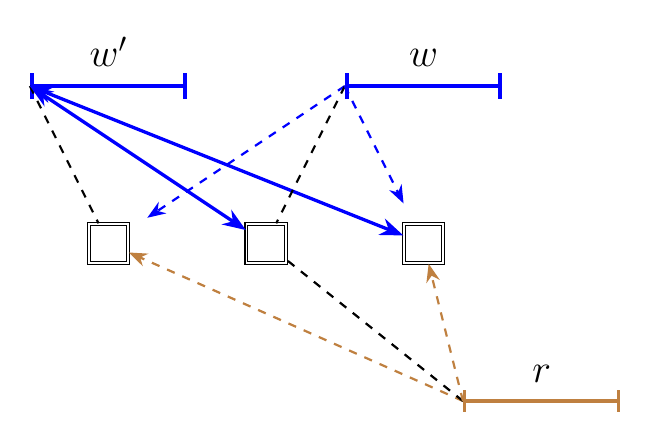
\begin{tikzpicture}[
  comm/.style = {>=Stealth, <->, blue, very thick}, 
  nocomm/.style = {thick, dashed},
  noack/.style = {>=Stealth, ->, thick, blue, dashed}]

  % ops: w', w, and r
  \itv{(0,0)}{(2,0)}{w'}{ultra thick, blue}
  \itv{(4,0)}{(6,0)}{w}{ultra thick, blue}
  \itv{(5.5,-4)}{(7.5,-4)}{r}{very thick, brown}

  % 3 bins
  \foreach \x in {1, 3, 5} {
    \node (\x) [double, rectangle, draw, minimum size = 0.50cm] at (\x, -2) {};
  }

  % w' sends balls into bins
  \draw[nocomm] (start w') to (1);
  \draw[comm] (start w') to (3);
  \draw[comm] (start w') to (5);

  % r sends balls into bins
  \draw[noack, brown] (start r) to (1);
  \draw[nocomm] (start r) to (3);
  \draw[noack, brown] (start r) to (5);

  % w sends balls into bins
  \draw[noack, shorten >= 8pt] (start w) to (1);
  \draw[nocomm] (start w) to (3);
  \draw[noack, shorten >= 8pt] (start w) to (5);
\end{tikzpicture}
\end{document}